%%%%%%%%%%%%%%%%%%%%%%%%%%%%%%%%%%%%%%%%%%%%%%%%%%%%%%%%%%%%%%%%%%%%%
% 																    %
% 	Class pgffigure for easier plots using pgfplots					%
%																	%
%	Possible options:												%
%   nofinal|final - draws 1cm grid on background or 				%
%                   disables grid. final by default.				%
%   nocyr|cyr - usage western or cyrillic numbers notation:			%
%               cyr enables comma `,' instead of dot `.' and		%
%               removes dot as thouthands separator.				%
%               nocyr by default.									%
%																	%
%																	%
%%%%%%%%%%%%%%%%%%%%%%%%%%%%%%%%%%%%%%%%%%%%%%%%%%%%%%%%%%%%%%%%%%%%%

\documentclass[final]{pgffigure}
\usepackage[utf8]{inputenc}
\usepackage{mathrsfs}
\usepackage{xcolor}

\pagestyle{empty}

\renewcommand{\vec}[1]{\bm{#1}}

\usetikzlibrary{patterns,fit}
\usepgfplotslibrary{fillbetween}

% colors definition
\definecolor{colj0}{HTML}{D73240}
\definecolor{colj1}{HTML}{00E745}
\definecolor{colj2}{HTML}{A600F2}
\definecolor{colj3}{HTML}{FC9A0E}
\definecolor{colj4}{HTML}{0000F2}

\begin{document}
	
	\begin{tikzpicture}[helpgrid]
		\small
		% text on stripe
		\node at (0,0) {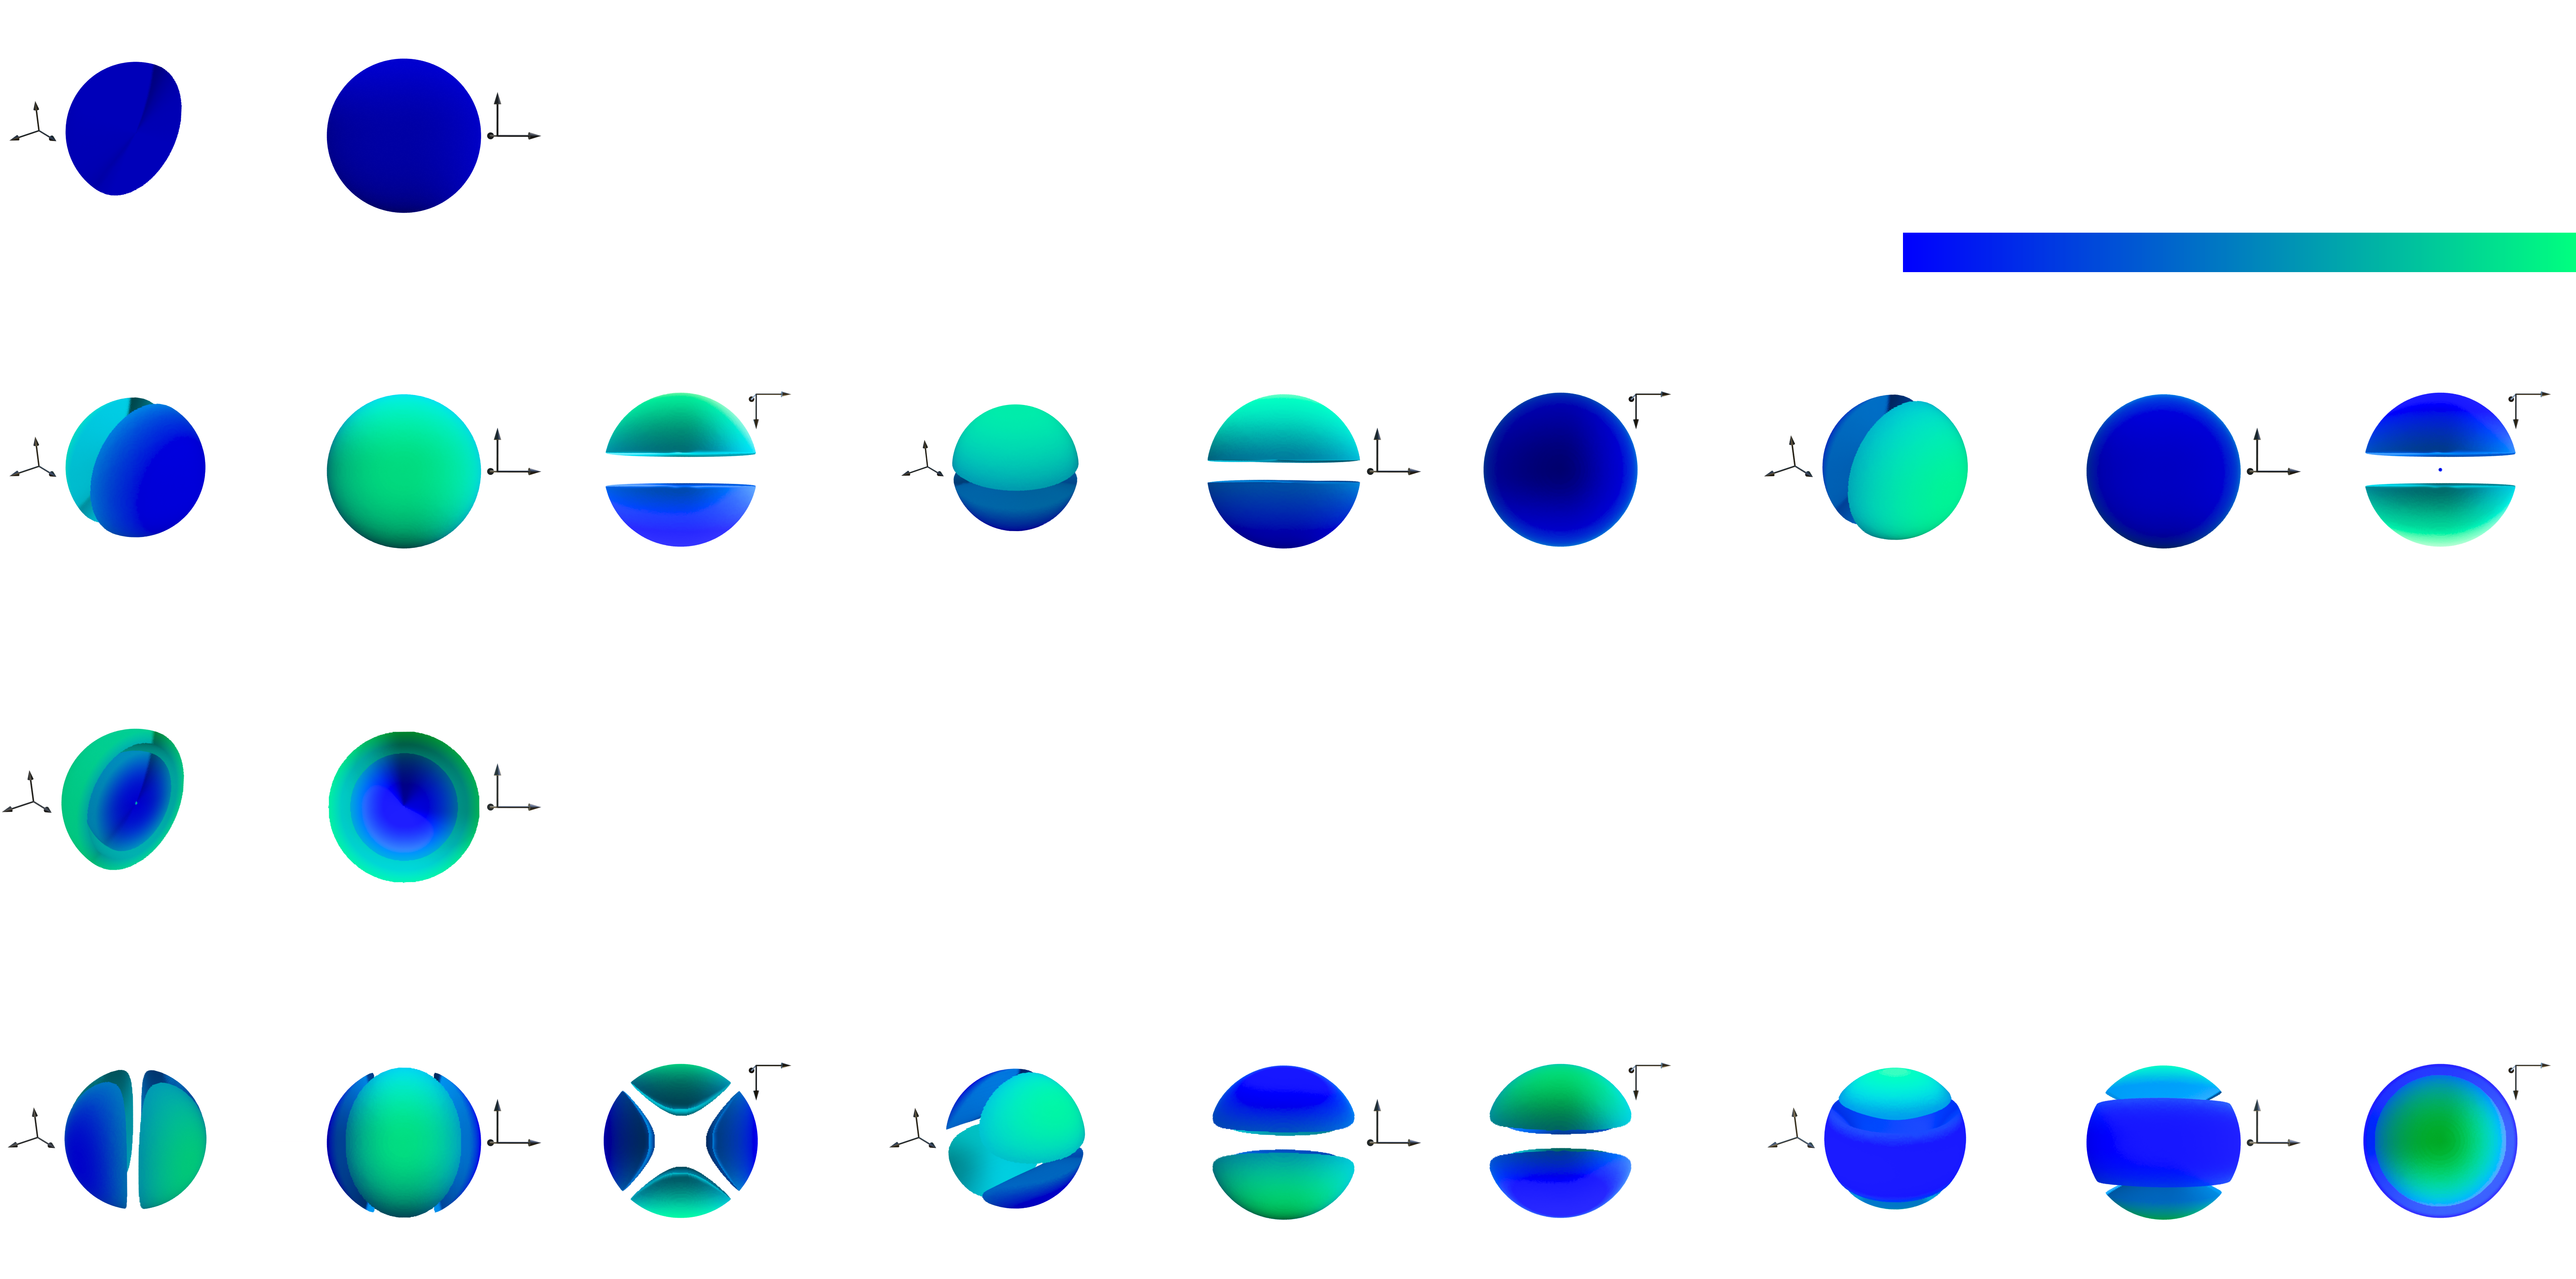
\includegraphics[width=\textwidth]{modes.png}};
		% legend 
		\node at (3, 2.1) { $\text{min}$ };
		\node at (6, 2.1) { $\text{max}$ };
		% n
		\node at (-6.8, 2.5) { $n = 0$ };
		\node at (-6.8, 0.9) { $n = 1$ };
		\node at (-6.8, -1.5) { $n = 2$ };
		% l m
		% n = 0 l = 0 
		\node at (-4.9, 1.8) { $l = 0, m = 0$ };
		% n = 1 l = 1
		\node at (-4.9, 0.1) { $l = 1, m = 1$ };
		\node at (0, 0.1) { $l = 1, m = 0$ };
		\node at (4.2, 0.1) { $l = 1, m = -1$ };
		% n = 2 l = 0
		\node at (-4.9, -1.4) { $l = 0, m = 0$ };
		% n = 2 l = 2
		\node at (-4.9, -3.1) { $l = 2, m = 2$ };
		\node at (0, -3.1) { $l = 2, m = 1$ };
		\node at (4.2, -3.1) { $l = 2, m = 0$ };
		
		
	\end{tikzpicture}
	
\end{document}

